\section{Specification requirements}

\subsection{Functional requirements} % (fold)
\label{sub:Functionalrequirements}

\paragraph{Graphical User Interface}
\begin{itemize}
    \item When the user first opens the application he is met
        by an ``Employees'' category view. At the bottom of the screen
        a bar with three buttons with icon and
        description (``Employees'', ``Departments'' and
        ``Projects'') is shown. From here the user can tab the buttons to change
        the content of the list above.

    \item The ``Employees'' category is a list of all the
      employees. The employees are sorted by either first or last
      name, selected by a button at the top of the interface. Next to
      every employee name there is a small picture of them to aid
      identification. If there are ever less than 30 employees in a
      list, grouping on the first letter will not be used, to give the
      user a less cluttered view. There should be a coloured overlay to
      show if the user is available, maybe available or not available
      (green/yellow/red).

    \item The ``Departments'' and ``Projects'' categories shows a list
      of all departments/projects, sorted by name.  A user can tap on
      any one of these, and will then be shown an ``Employees''
      category listing only the employees tied to that particular
      employee group.

    \item When displaying an employees list with a department or project,
      the main area where involved people are sitting should be displayed.

    \item When an employee has been selected, the S7Finder app shows
      the user a profile view of the employee. This view contains a
      large picture of the employee, their name, phone number, job
      title, department, a listing of projects they're involved in and
      desk location
        \footnote{Desk location is a number indicating the exact
          placement of an employees desk, and an image showing the
          main area of the floor, with the location marked. If this desk location
          does not match a known image, an unknown location image is shown.}
      , and availability status
        \footnote{Availability statuses consist of a display showing a
          status from an Exchange service (available, at lunch, sick,
          vacation etc.).}.

	\item When the desk location is tapped it should open up in a
      larger view.

    \item When the S7Finder app is not in use, it displays a pause
      screen containing the floor number and the text "People Finder".

    \item If the application gets in an error state, it should display
      an "out of order" screen.

    \item The screen should turn black at night at specified hours.

\end{itemize}

\paragraph{Application data and configuration}
\begin{itemize}
\item S7Finder has a config file that is requested from a central
  server at intervals set by the config file provided from the server,
  or by default, every night. When the iPad connects to the web
  service to acquire the config file, it provides the iPads MAC
  address as a UUID (Universally Unique ID).  The web service returns
  an XML file with the following data:
  \begin{itemize}
  \item Screen turning black hours
  \item Interval for retrieving employee data
  \item Interval for retrieving config files
  \item Interval for checking for new images
  \item iPad Location floor
  \item Base URL for fetching all data (including config and images)
  \item Seconds before going back to Standby Screen
  \item The default sort method for the employee list (First Name or
    Last Name)
  \item The sequence of letters displayed on the right of the employee
    list
  \end{itemize}

\item To keep the data up to date, the S7Finder app requests updates
  (in XML) from a web service every 5-10 minutes. The interval can be
  changed through the config file.  It will also request an update
  when a user activates the app, to ensure that the data displayed is
  up-to-date.
\end{itemize}

\subsection{Non-functional requirements} % (fold)
\label{sub:Non-functional requirements}

\paragraph{Quality requirements} % (fold)
\label{ssub:Quality requirements}

\begin{enumerate}
\item Any user must be able to locate a specific employee within 1
  minutes, without prior training or experience with the
  system. [Usability requirement]
\item The information displayed by the system must be presented in a
  clear and concise way. [Usability requirement]
\item There must be no noticeable latency when using the system. All
  the different views of the application must be shown within 0.5
  seconds. [Performance requirement]
\item The user interface elements must be of a size, so that
  non-experienced tablet users still fell comfortable with the
  app. [Usability requirement]
\end{enumerate}

We are aware that the quality requirements should be measurable in
order to assert that the final product conforms to these, but due to
the scope of the project we acknowledge that we are unable to do
research sufficient to determine reasonable values for list items 2
and 4. Further, should we be able to determine reasonable values for
these requirements, we would still be unable to test these to the
amount required for statistical correctness.

\paragraph{Constraints} % (fold)
\label{ssub:Constraints}

\begin{itemize}
    \item The system must be written on the .NET
      platform. [Implementation requirement]
    \item The system must run on (minimum requirement) an iPad 2 with
      iOS version 5.1. [Implementation requirement]
    \item All code documentation must be written in the standard .NET
      format using XML. [Implementation requirement]
    \item The user interface must include the company branding. [User
      Interface Requirement]
    \item The status codes used for the app should be the same as the
      ones used in the company Exchange service. [Implementation
        requirement]
\end{itemize}

The client (Subsea7) will be responsible for installation and
maintenance, including encasing the iPad to stop end-users from
exiting the application. \footnote{The Apple iPad features a ``home''
  button on the bottom of the device, which returns the user to the
  desktop.  As the functionality of this button is impossible (within
  reasonable limits) to override, it's necessary to provide a physical
  barrier to avoid a user pressing this button.}

\subsection{Use case overview}

In \fref{fig:ucoverview} all our use cases are shown. We have two
users, the regular user of our application \texttt{Person} and the
\texttt{Administrator}. The administrator is a developer working for
Subsea7, who has access to an administration interface.

\begin{figure}[!h]
    \centerline{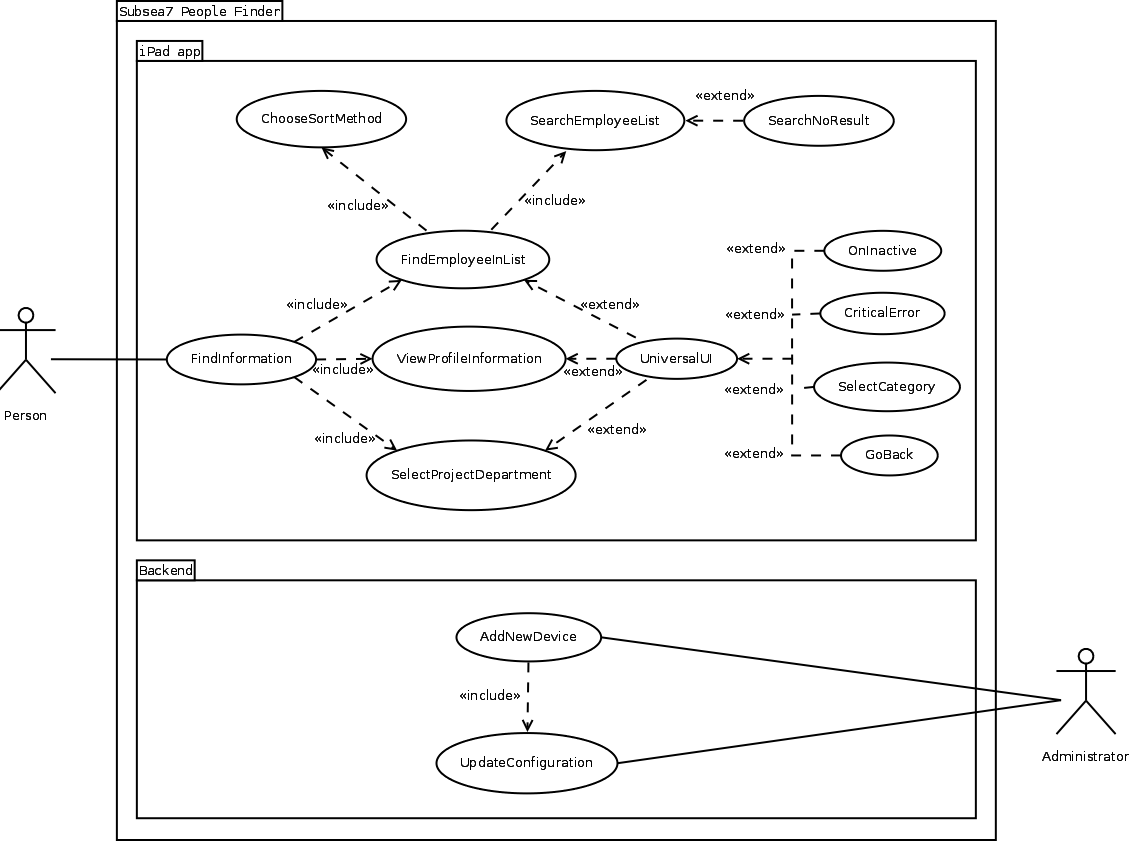
\includegraphics[width=1\textwidth]{use_case_overview}}
    \caption{Use case overview}
    \label{fig:ucoverview}
\end{figure}

\clearpage

%
% New commands for layout in use cases
%
\newcommand{\usecaseline}{\vspace*{-6pt} \noindent
  \rule[0.5ex]{1\columnwidth}{1pt} \vspace*{-16pt}}
\newcommand{\usecasethickline}{\vspace*{-6pt} \noindent
  \rule[0.5ex]{1\columnwidth}{1.5pt} \vspace*{-16pt}}

\subsection{Use Cases} \label{sec:usecases}

\subsubsection{Use case 1: FindEmployeeInList}

\usecasethickline

\begin{description}[style=multiline,leftmargin=4cm,font=\normalfont]
\item[\emph{Use case name:}] FindEmployeeInList \footnote{This use
    case's sequence diagram is shown in \autoref{fig:uc1} on
    \autopageref{fig:uc1}}
\end{description}

\usecaseline

\begin{description}[style=multiline,leftmargin=4cm,font=\normalfont]
    \item[\emph{Paticipating actors:}] \texttt{Person}.
\end{description}

\usecaseline

\begin{description}[style=multiline,leftmargin=4cm,font=\normalfont]
    \item[\emph{Flow of events}]
        \begin{enumerate} [style=multiline,leftmargin=1.5em,font=\normalfont]

            \item {\leftskip4em \texttt{S7Finder} presents a table containing a row
              for all employees (possibly filtered on a project or
              department.  For each employee in there is a
              thumbnail-picture (with a coloured overlay indicating
              the availability of the employee), their full name,
              title, department, location is also shown.  At the top
              of the screen there is a switchbutton with the text
              "sort by: Firstname $|$ Lastname".  Just above the table
              a search bar is displayed.

            }

            %{\leftskip0em
          \item \texttt{Person} can at any time use the switchbutton,
            invoke the use case \texttt{ChooseSortMethod}.
            %}

          \item \texttt{Person} uses his finger to scroll up and down
            the list to find the employee he is looking for, or uses
            the \texttt{SearchEmployeeList} use case. When
            \texttt{Person} finds an employee meeting the criteria he
            is looking for, he taps the row with the employee.

        
        \end{enumerate}

\end{description}

\usecaseline

\begin{description}[style=multiline,leftmargin=4cm,font=\normalfont]
\item[\emph{Entry condition}] The \texttt{Person} has selected the top
  level category for all employees, or a specific project or
  department.
\end{description}

\usecaseline

\begin{description}[style=multiline,leftmargin=4cm,font=\normalfont]
\item[\emph{Exit conditions}] The \texttt{Person} has selected an
  employee meeting the requirements he was looking for.
\end{description}

\usecaseline

\begin{description}[style=multiline,leftmargin=4cm,font=\normalfont]
\item[\emph{Quality requirements}] A Person must be able to locate an
  employee meeting the requirements he was looking for within 1
  minutes, without prior training or experience with the system.
\end{description}

\usecasethickline
\clearpage


%%%%%%%%%%%%%%%%%%%%%%%%%%
%   Use case 2: GoBack   %
%%%%%%%%%%%%%%%%%%%%%%%%%%


\subsubsection{Use case 2: GoBack}

\usecasethickline

\begin{description}[style=multiline,leftmargin=4cm,font=\normalfont]
\item[\emph{Use case name:}] GoBack\footnote{This use case's sequence
    diagram is shown in \autoref{fig:uc2} on \autopageref{fig:uc2}}
\end{description}

\usecaseline

\begin{description}[style=multiline,leftmargin=4cm,font=\normalfont]
\item[\emph{Paticipating actors:}] \texttt{Person}
\end{description}

\usecaseline

\begin{description}[style=multiline,leftmargin=4cm,font=\normalfont]
    \item[\emph{Flow of events}]
         \begin{enumerate}[style=multiline,leftmargin=1.5em,font=\normalfont]
             \item \texttt{Person} taps the back button  located in the
                 upper left corner of the screen.

            {\leftskip4em
            \item \texttt{S7Finder} respond be presenting the previous screen.

            }
       \end{enumerate}
\end{description}

\usecaseline

\begin{description}[style=multiline,leftmargin=4cm,font=\normalfont]
            \item[\emph{Entry condition}]
                This use case extends any other use case that takes \texttt{Person} one level down in the application.
\end{description}

\usecaseline

\begin{description}[style=multiline,leftmargin=4cm,font=\normalfont]
    \item[\emph{Exit conditions}]
    \texttt{Person} has been taken one level up in the view stack.
\end{description}

\usecaseline

\begin{description}[style=multiline,leftmargin=4cm,font=\normalfont]
    \item[\emph{Quality requirements}] None.
\end{description}

\usecasethickline
\clearpage

%%%%%%%%%%%%%%%%%%%%%%%%%%%%%%%%%%%%%%
%   Use case 3: SearchEmployeeList   %
%%%%%%%%%%%%%%%%%%%%%%%%%%%%%%%%%%%%%%

\subsubsection{Use case 3: SearchEmployeeList}

\usecasethickline

\begin{description}[style=multiline,leftmargin=4cm,font=\normalfont]
    \item[\emph{Use case Name:}]SearchEmployeeList\footnote{This use case's sequence diagram is shown in \autoref{fig:uc3} on \autopageref{fig:uc3}}
\end{description}

\usecaseline

\begin{description}[style=multiline,leftmargin=4cm,font=\normalfont]
    \item[\emph{Paticipating actors:}] \texttt{Person}
\end{description}

\usecaseline

\begin{description}[style=multiline,leftmargin=4cm,font=\normalfont]
    \item[\emph{Flow of events}]
         \begin{enumerate}
             \item \texttt{Person} tabs the search field

            {\leftskip4em
            \item \texttt{S7Finder} responds by removing the
              switchbutton with the text "sort by: Firstname $|$
              Lastname" from the top right, removing the back button
              (if present) and adding a cancel button to the top left
              of the screen with the text ``Cancel''. A virtual
              keyboard is added to lowest area of the screen.

              % The empty line bewteen the text and the } has to be
              % there, do not ask me why.. //j0br
            }
          \item \texttt{Person} starts typing in the firstname,
            middelname or lastname of the employee he is looking for.

            {\leftskip4em
            \item On each key stroke \texttt{S7Finder} updates the
              list, so it only contains employees' whose names
              (first/middle/last) begins with the search text.

              % The empty line bewteen the text and the } has to be
              % there, do not ask me why.. //j0br
            }
          \item \texttt{Person} may scroll though the list to find the
            employee he is looking for, and may hide the keyboard.

       \end{enumerate}

\end{description}

\usecaseline

\begin{description}[style=multiline,leftmargin=4cm,font=\normalfont]
\item[\emph{Entry condition}] \texttt{Person} is on the employee list
  screen, and knows at least part of the name for the employee he is
  looking for.
\end{description}

\usecaseline

\begin{description}[style=multiline,leftmargin=4cm,font=\normalfont]
    \item[\emph{Exit conditions}]
        \texttt{Person} has found the employee he is looking for (also see SearchNoResult).
\end{description}

\usecaseline

\begin{description}[style=multiline,leftmargin=4cm,font=\normalfont]
    \item[\emph{Quality requirements}]
  The employee must be found within 30 seconds.
\end{description}

\usecasethickline

\bigskip

\subsection{Class diagram}
The class diagram is shown in \fref{fig:decomp-class_diagram}. Some methods have been omitted for simplicity
(E.g.\ for the GUI \texttt{ViewWillAppear}, \texttt{ViewDidAppear}, \texttt{ViewWillDisappear}, \texttt{ViewDidDisappear} \texttt{PrepareForSegue} \@).
Relationships to the Utility and Config classes have also been removed for brevity. For a complete description
of all parts of the class diagram, please see \autoref{sub:sd-subsystem_decomposition}.

\begin{sidewaysfigure}
    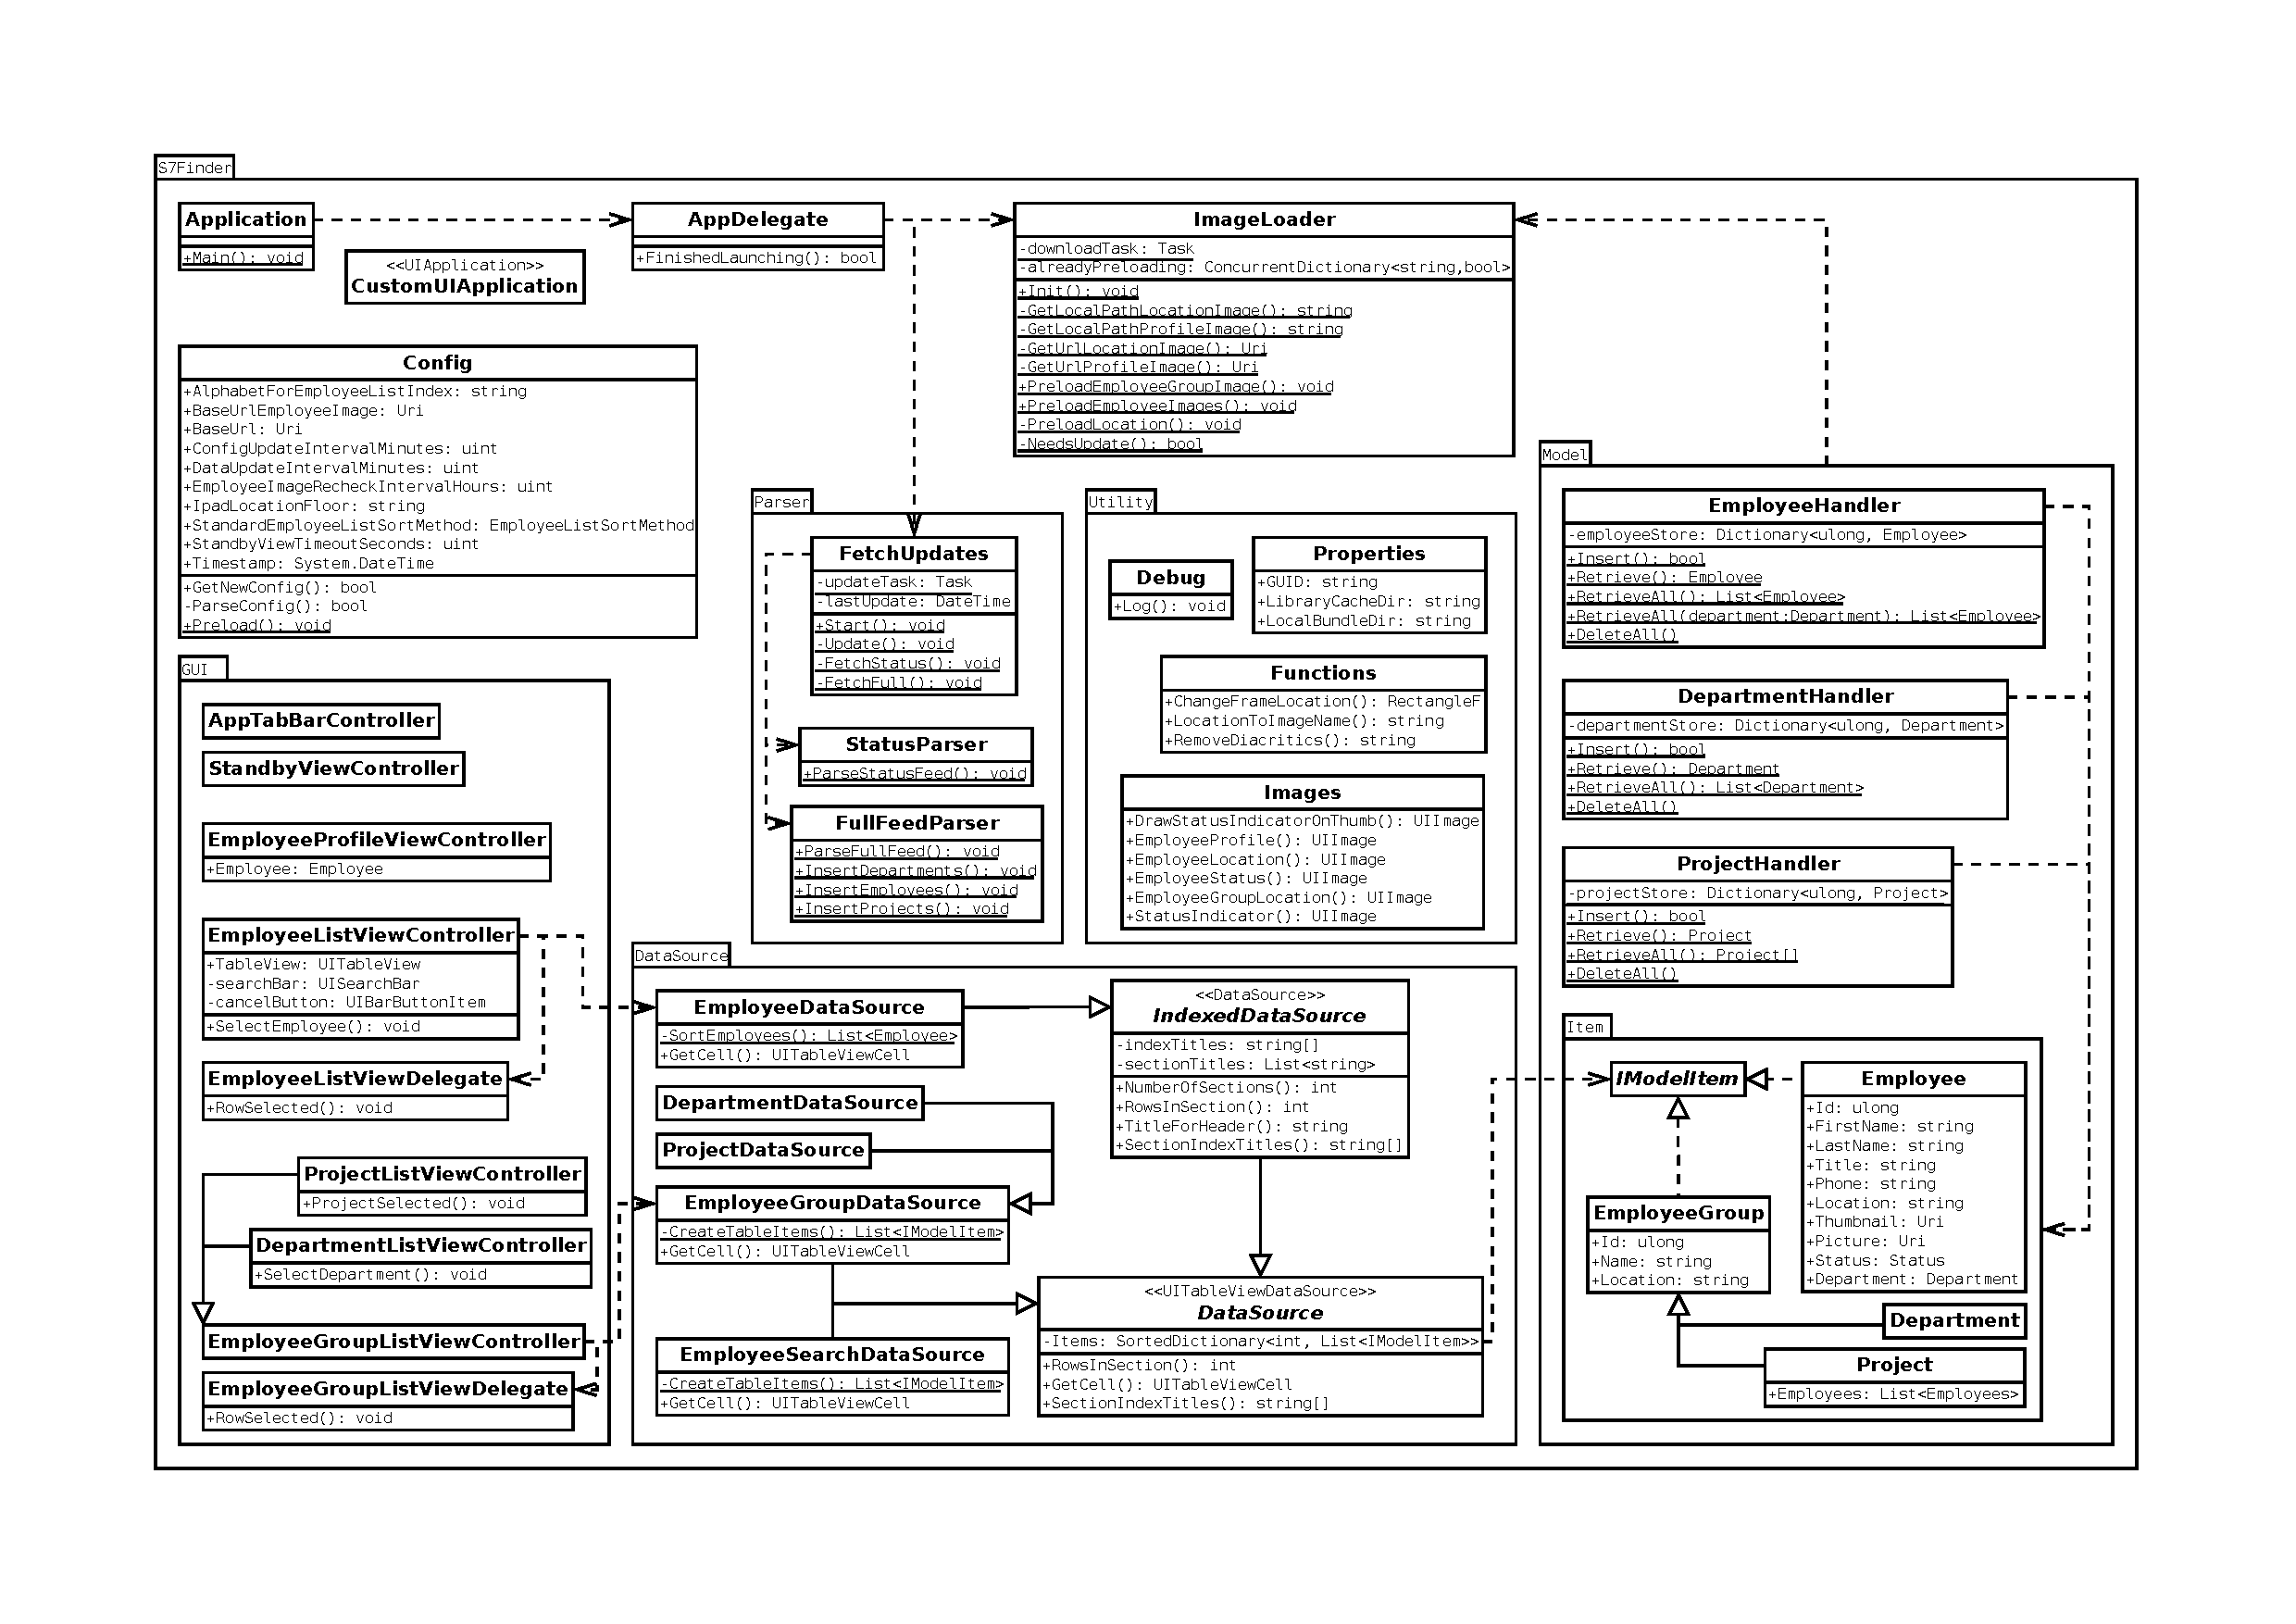
\includegraphics[width=\textwidth]{class_diagram}
    \caption{For a complete description of all parts of the class diagram,
        please see \autoref{sub:sd-subsystem_decomposition}}
    \label{fig:decomp-class_diagram}
\end{sidewaysfigure}

\newpage
\subsection{Sequence Diagrams}

The sequence diagrams for the three use cases described in section \ref{sec:usecases} are shown below. Objects marked with a grey background are part of the iOS API.

\subsubsection{Sequence diagram 1: FindEmployeeInList}

\begin{figure}[h!]
    \centerline{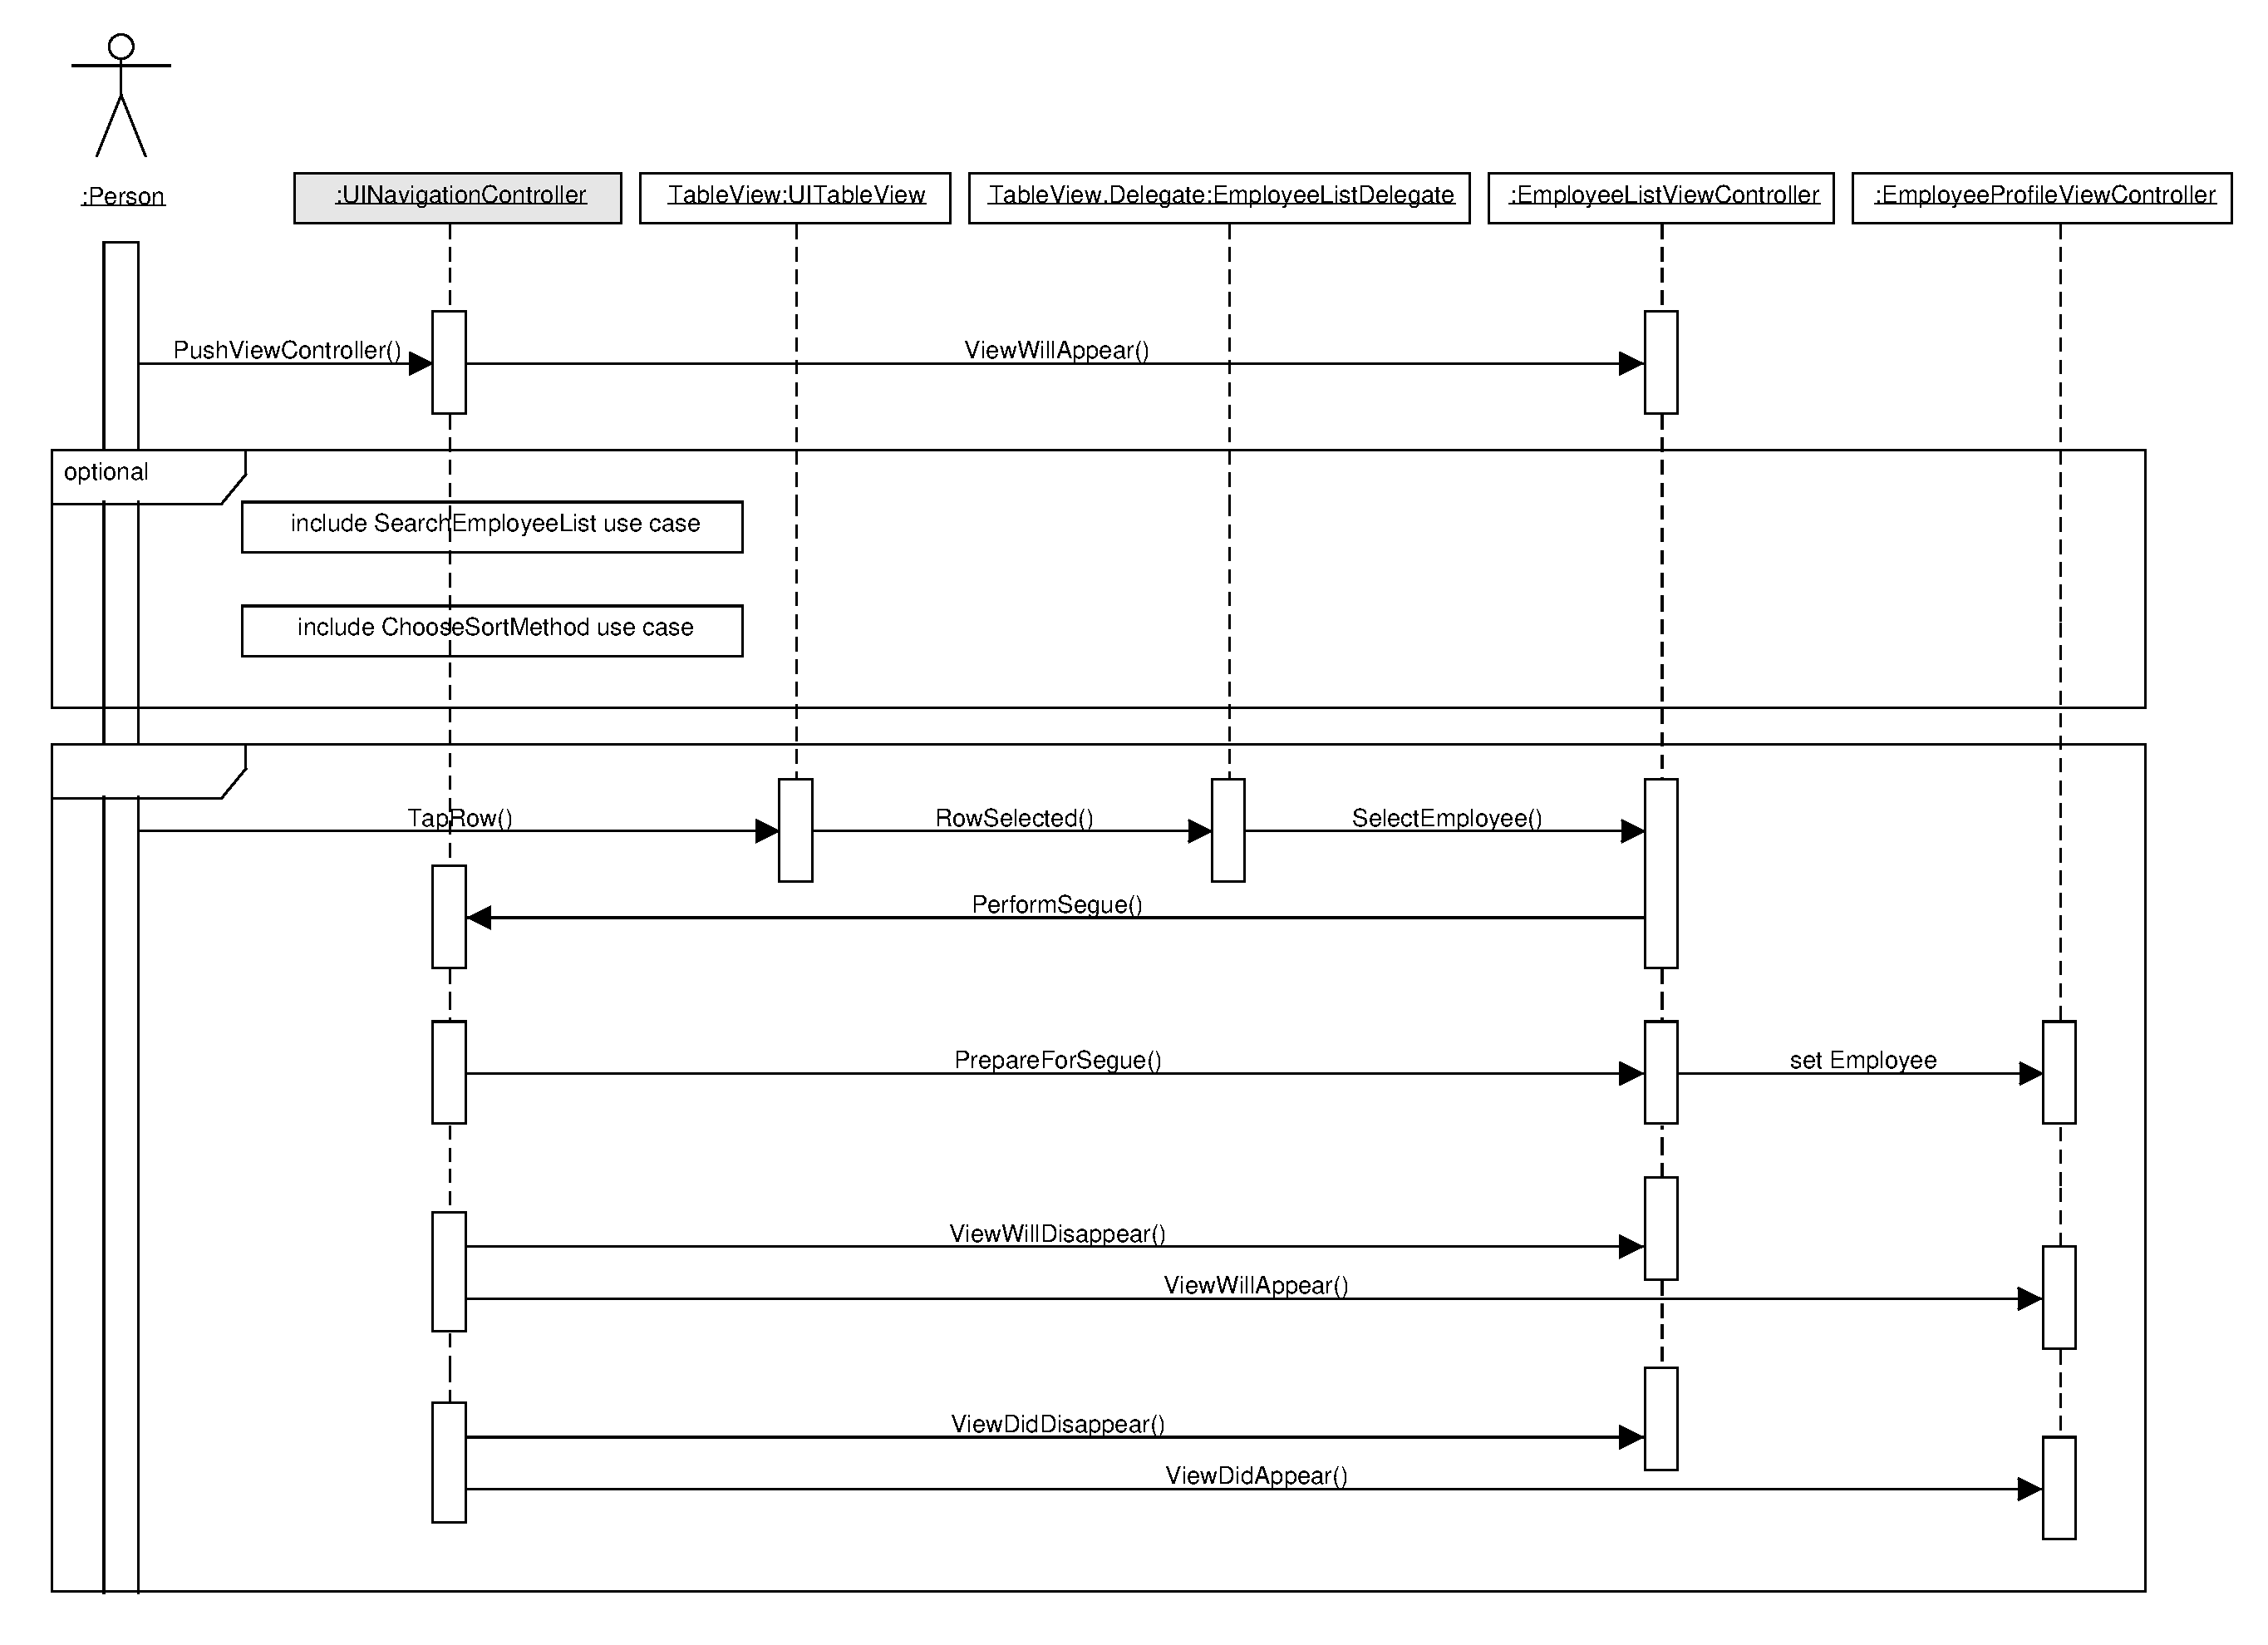
\includegraphics[width=1\textwidth]{seq_find}}
    \caption{Sequence diagram of use case FindEmployeeInList}
    \label{fig:uc1}
\end{figure}

In \fref{fig:uc1} the \texttt{TableView} is a property of the \texttt{UIEmployeeListViewController}. The lower part of the diagram has been inserted into a interaction frame, because all these events are started by the \texttt{TapRow}.

\subsubsection{Sequence diagram 2: GoBack}

\begin{figure}[H]
    \centerline{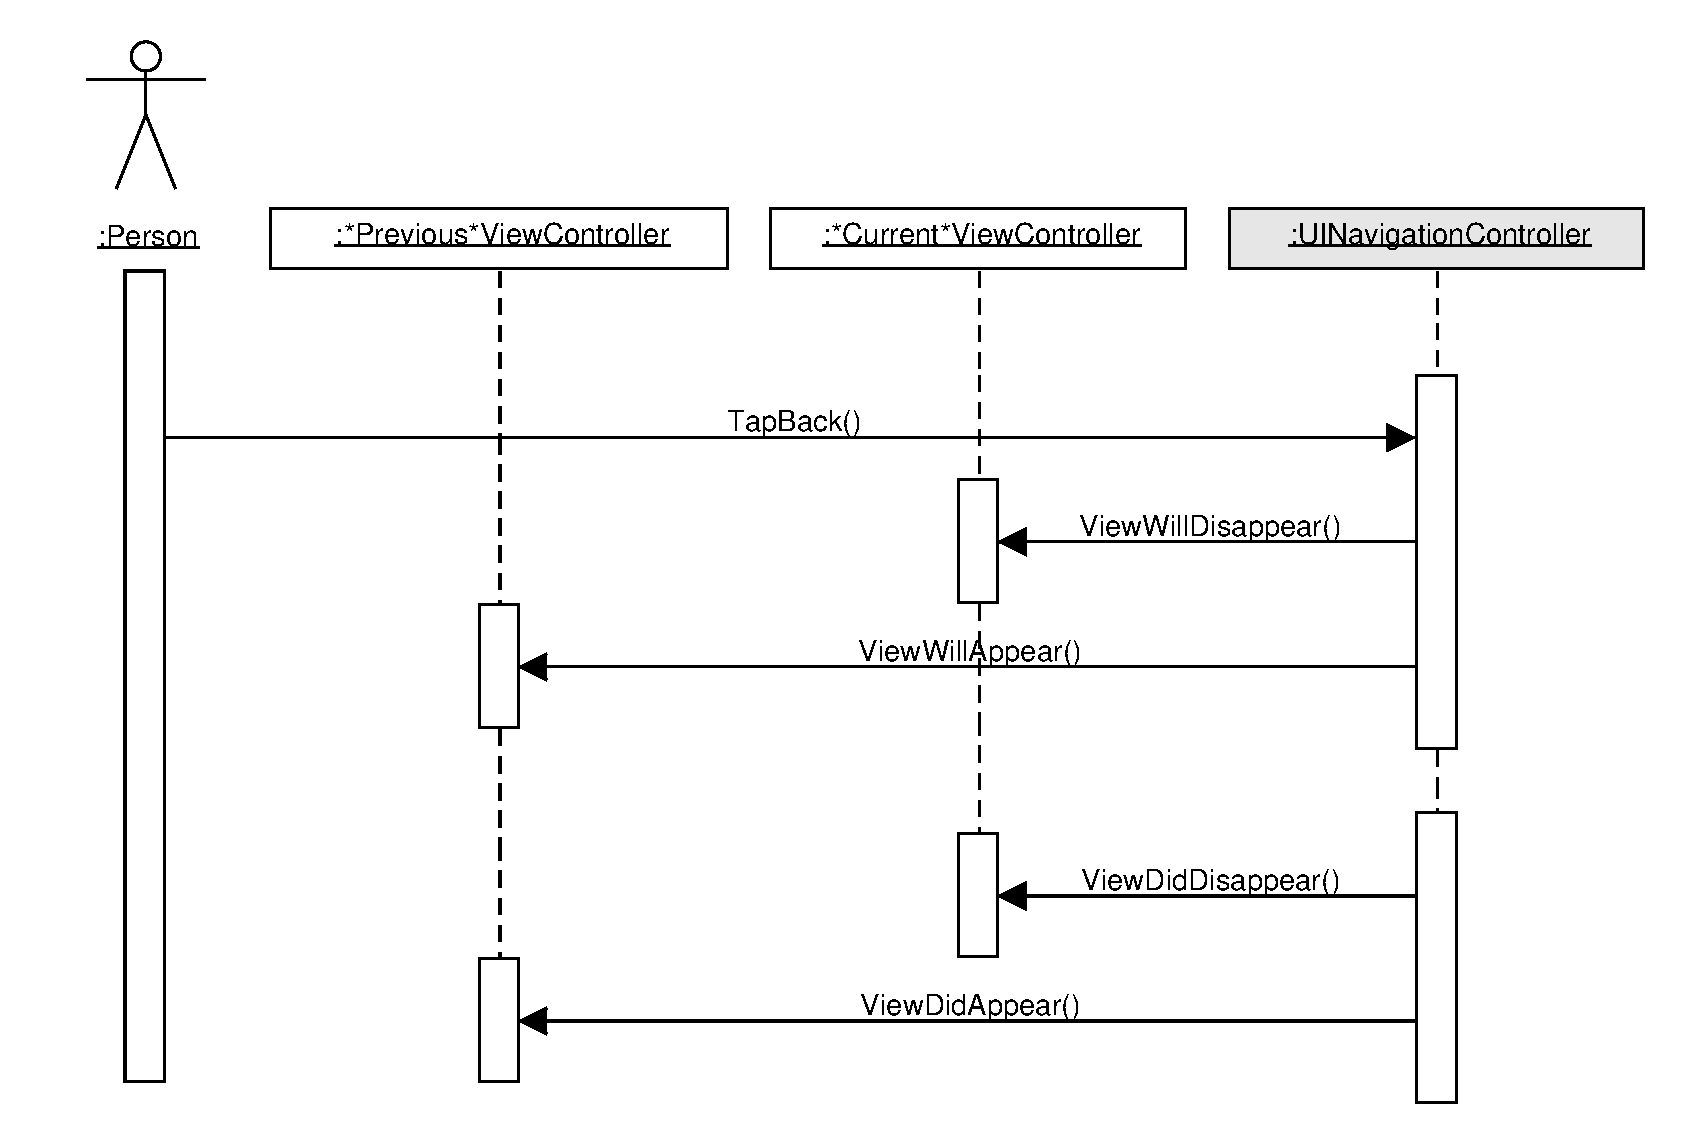
\includegraphics[width=1\textwidth]{seq_back}}
    \caption{Sequence diagram of use case GoBack }
    \label{fig:uc2}
\end{figure}

In \fref{fig:uc2} \texttt{*Previous*ViewController} and \texttt{*Current*ViewController} are placeholders for the actual \texttt{ViewControllers}, and is just used here to show the event flow.

\newpage
\subsubsection{Sequence diagram 3: SearchEmployeeList}

\begin{figure}[H]
    \centerline{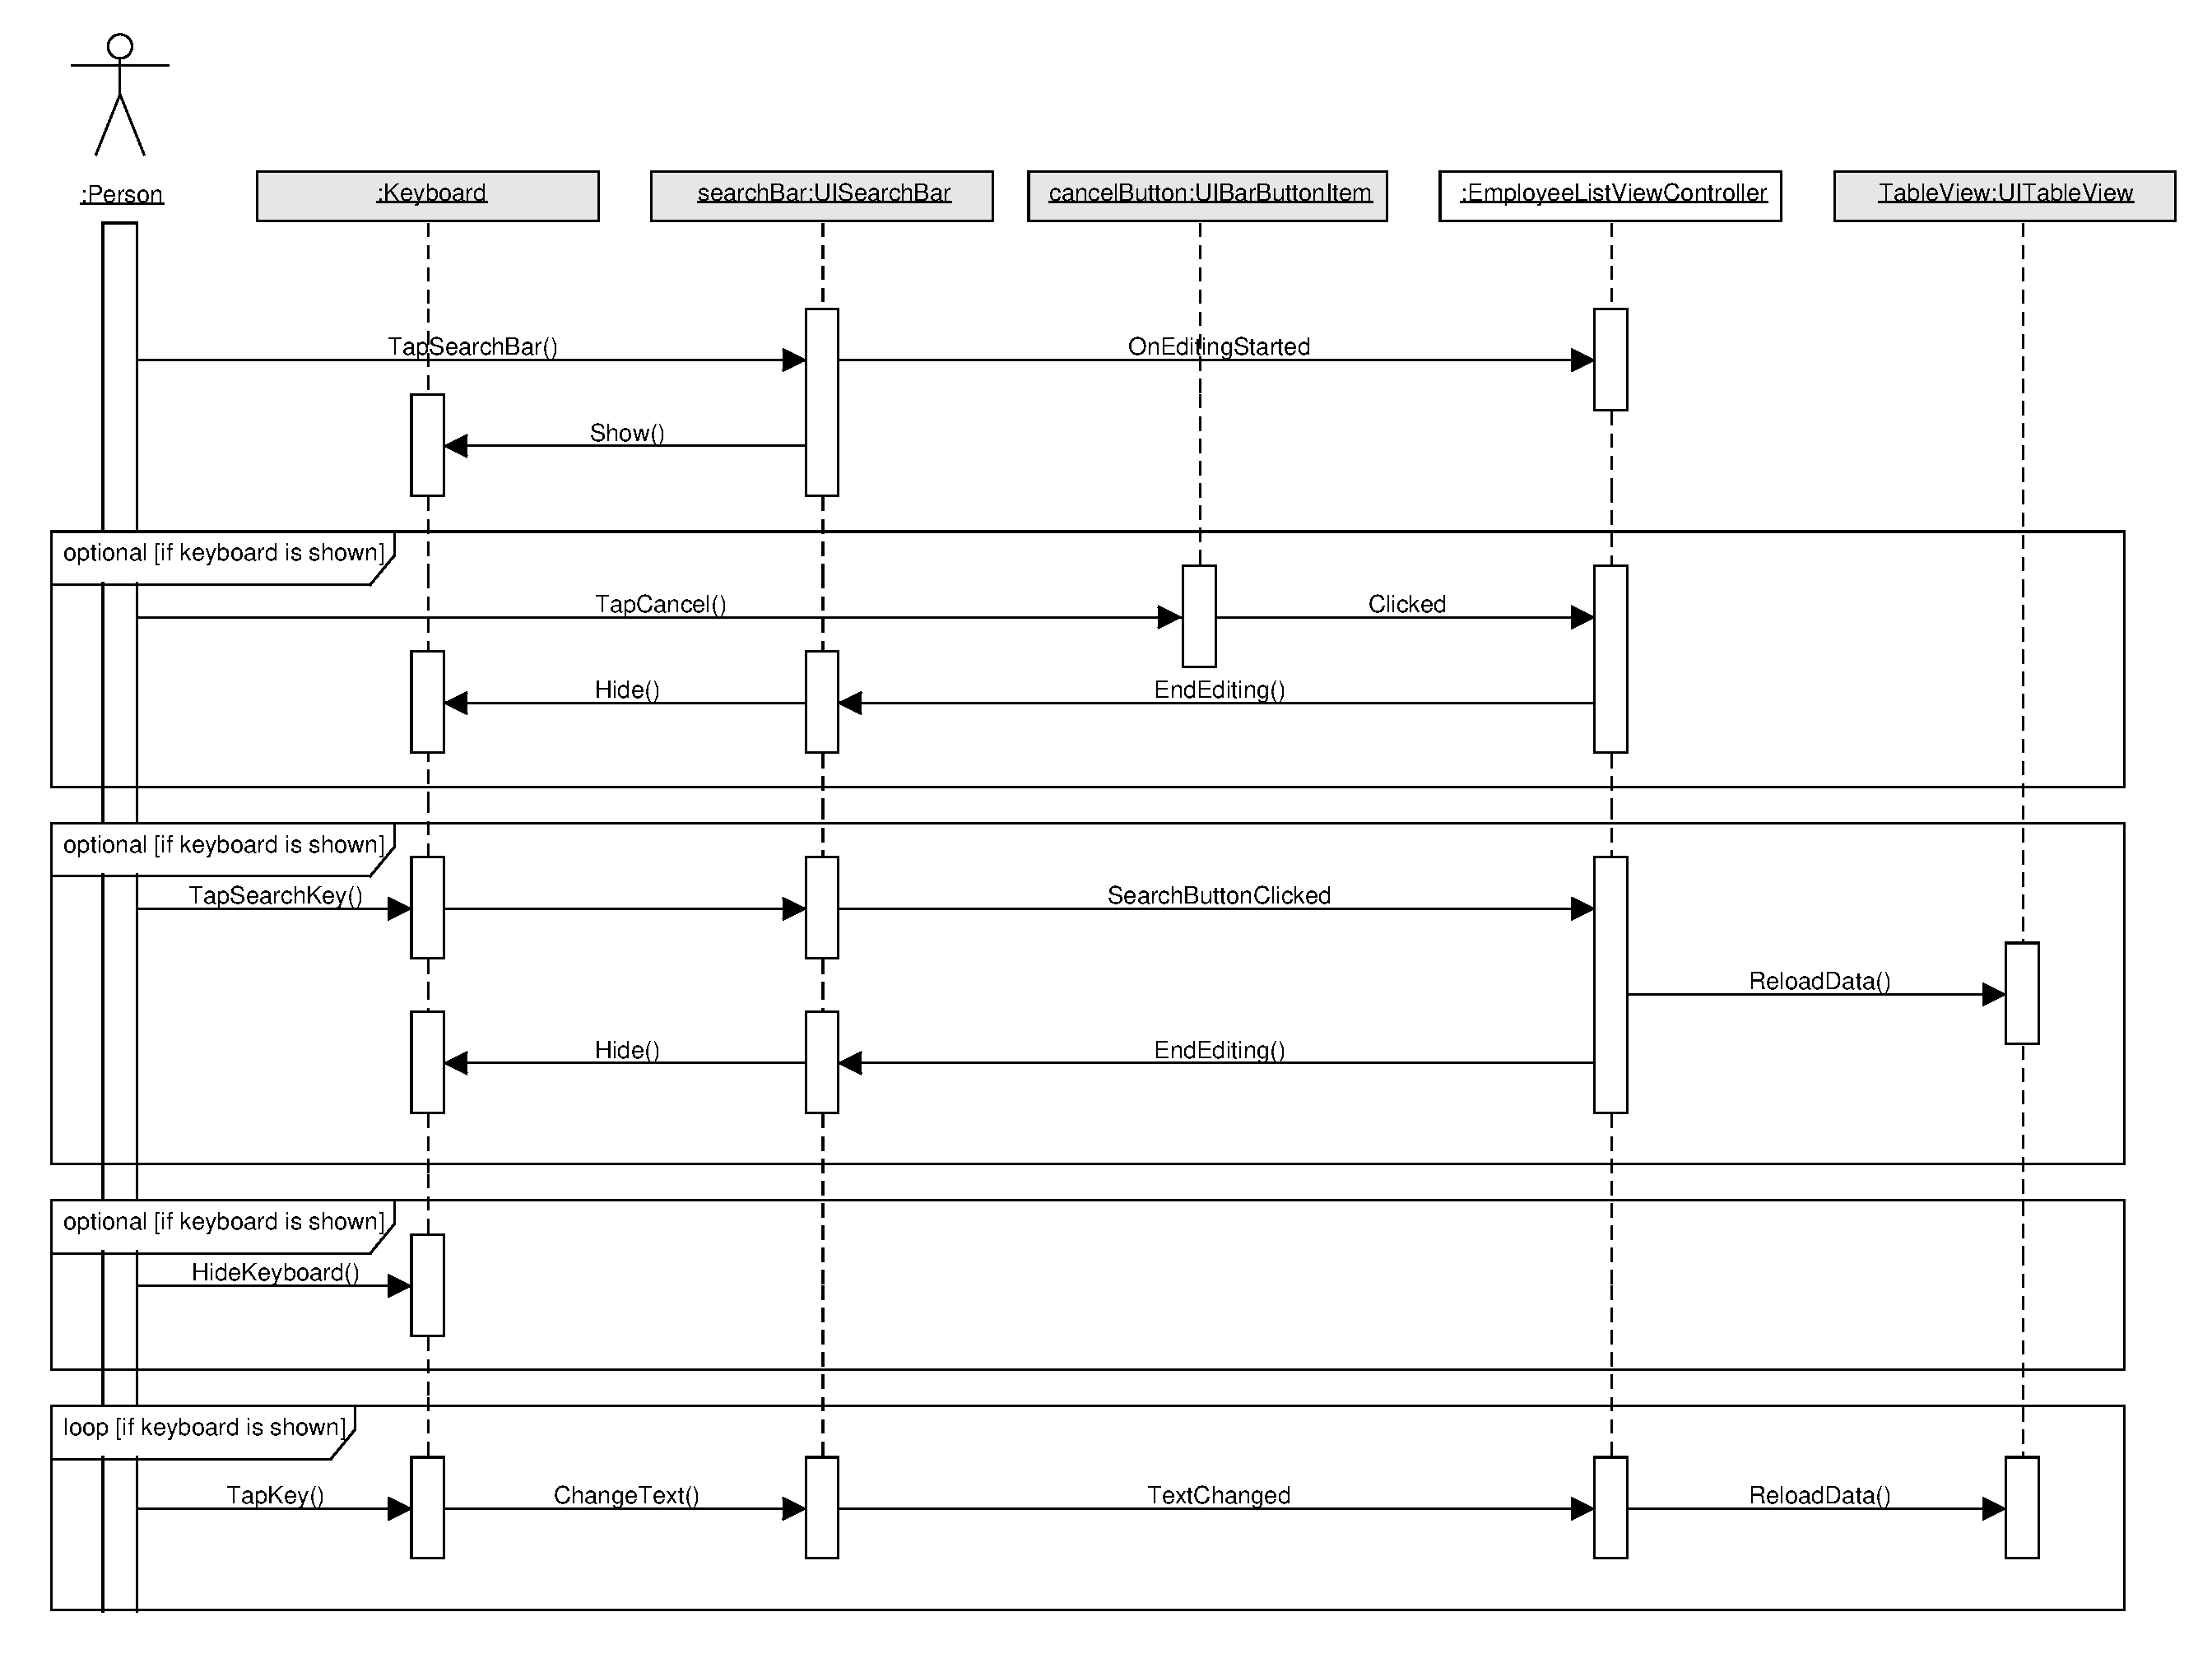
\includegraphics[width=1\textwidth]{seq_search}}
    \caption{Sequence diagram of use case SearchEmployeeList}
    \label{fig:uc3}
\end{figure}

In \fref{fig:uc3} the three optional and the loop sequence can be executed in any order and several times.
